\documentclass[11pt,a4paper,oneside]{report}
\usepackage{iftex}
\ifPDFTeX
  \usepackage[utf8]{inputenc}
\fi
\usepackage[T1]{fontenc}
\usepackage{lmodern}
\usepackage[spanish,es-nodecimaldot,es-lcroman]{babel}
\usepackage[margin=2.5cm,headheight=15pt]{geometry}
\usepackage{microtype}
\usepackage{amsmath,amssymb}
\usepackage{booktabs,longtable,tabularx,array}
\usepackage{graphicx}
\usepackage{xcolor}
\usepackage{enumitem}
\usepackage{listings}
\usepackage{tikz}
\usetikzlibrary{arrows.meta,positioning}
\usepackage{fancyhdr}
\usepackage{xurl}
\usepackage{hyperref}
\usepackage{bookmark}
\definecolor{azul}{HTML}{1D4ED8}
\definecolor{tinta}{HTML}{14243B}
\definecolor{fondo}{HTML}{F5F7FB}
\hypersetup{hypertexnames=false,colorlinks=true,linkcolor=tinta,urlcolor=azul,citecolor=azul,
  pdftitle={Memoria técnica: abandono bancario y decisiones de retención},
  pdfauthor={Darwin Jacome Cuenca},pdfsubject={Documentación de bank-churn-ml v1.0.1}}
\graphicspath{{../../reports/figures/}}
\pagestyle{fancy}
\fancyhf{}
\fancyhead[L]{\small bank-churn-ml}
\fancyhead[R]{\small Memoria técnica de la entrega v1.0.1}
\fancyfoot[C]{\thepage}
\setcounter{tocdepth}{1}
\setcounter{secnumdepth}{2}
\setlength{\parskip}{0.35em}
\setlength{\emergencystretch}{2em}
\setlist[itemize]{itemsep=0.15em,topsep=0.3em}
\setlist[enumerate]{itemsep=0.2em,topsep=0.3em}
\renewcommand{\arraystretch}{1.18}
\newcolumntype{L}[1]{>{\raggedright\arraybackslash}p{#1}}
\newcommand{\versioncodigo}{9384e51}
\newcommand{\fuente}[1]{\par{\footnotesize\textit{Fuente:} \path{#1}.}\par}
\lstset{basicstyle=\ttfamily\footnotesize,backgroundcolor=\color{fondo},
  frame=single,rulecolor=\color{black!15},breaklines=true,columns=fullflexible,
  keepspaces=true,showstringspaces=false,tabsize=2,captionpos=b}

\begin{document}
\begin{titlepage}
\centering
{\large MEMORIA TÉCNICA DEL PROYECTO\par}
\vspace{2cm}
{\Huge\bfseries\color{tinta} Abandono bancario\par}
\vspace{0.4cm}
{\LARGE Decisiones de retención con probabilidades calibradas\par}
\vspace{1cm}
{\large Metodología estadística, modelado, decisión económica,\par
arquitectura, seguridad, operación y evidencia de entrega\par}
\vfill
{\Large Darwin Jacome Cuenca\par}
\vspace{0.5cm}
{\large Repositorio: \texttt{bank-churn-ml}\par}
{\large Entrega documentada: \texttt{v1.0.1}\par}
{\large Código de referencia: \texttt{\versioncodigo}\par}
\vspace{1cm}
{\large 15 de octubre de 2026\par}
\vspace{0.6cm}
\url{https://github.com/darwinjaco/bank-churn-ml}
\end{titlepage}

\pagenumbering{roman}
\chapter*{Resumen ejecutivo}
\addcontentsline{toc}{chapter}{Resumen ejecutivo}
El proyecto convierte una probabilidad de abandono bancario en una decisión
explícita de contacto. Su contribución no consiste únicamente en clasificar:
combina un modelo calibrado, una regla económica derivada de supuestos visibles,
explicaciones locales y una aplicación verificable. Se emplea el dataset público
\textit{Churn Modelling}, de 10\,000 clientes, con aproximadamente un 20,37\,\%
de abandono. La procedencia probablemente sintética y la falta de datos de
tratamiento limitan cualquier extrapolación a una institución real.

El desarrollo siguió siete especificaciones y decisiones preregistradas. Tras
comparar regresión logística, Random Forest y XGBoost, una regla de parsimonia
seleccionó Random Forest. La calibración sigmoidal se ajustó con predicciones
fuera de muestra de entrenamiento y se eligió en validación. El conjunto de
prueba se utilizó una sola vez, con modelo y política congelados.

En esa evaluación de 2\,000 clientes se registraron AP de 0,7047, ROC-AUC de
0,8616 y Brier de 0,1017. Bajo supuestos ilustrativos de valor de cliente de
1\,000 EUR, coste de contacto de 50 EUR y eficacia de retención del 30\,\%,
la política contacta a 634 clientes y obtiene 61\,600 EUR frente a 22\,100 EUR
por contactar a todos. Es una evaluación retrospectiva bajo supuestos, no
evidencia de ingresos realizados por una campaña.

La entrega incluye FastAPI, Streamlit, Docker, CI, auditoría de equidad, SHAP
y monitoreo simulado. Este último muestra un límite relevante: un cambio de
prevalencia puede deteriorar la calibración sin producir una alarma de cambio
en las entradas. La demo desplegada en Render fue comprobada mediante HTTPS,
controles de origen, subida protegida y navegación real. Esta memoria sintetiza
los artefactos existentes; su redacción no reentrena ni reevalúa la prueba.

\section*{Cómo leer la evidencia}
\begin{itemize}
\item \textbf{Desarrollo:} EDA, validación cruzada, selección, calibración,
  auditoría y simulaciones. No son estimaciones finales independientes.
\item \textbf{Prueba:} evaluación única del 7 de octubre de 2026, registrada
  en \path{reports/final_test.json} con \texttt{final=true}.
\item \textbf{Entrega:} código \texttt{\versioncodigo}, Release \texttt{v1.0.1},
  CI y comprobación pública documentados el 15 de octubre de 2026.
\end{itemize}
\tableofcontents
\listoftables
\listoffigures
\clearpage
\pagenumbering{arabic}

\chapter{Problema, alcance y gobierno del trabajo}
\section{Pregunta de negocio}
Con recursos de retención limitados, interesa decidir a qué clientes conviene
contactar. Una probabilidad elevada no basta si el coste de la acción supera
su valor esperado. El sistema responde tres preguntas: cuál es el riesgo de
abandono, si el contacto tiene valor esperado positivo y qué factores del modelo
explican la predicción. La salida combina probabilidad calibrada, decisión,
beneficio esperado y razones locales.

No se plantea una asignación bajo una cuota máxima de llamadas. La versión
entregada aplica un umbral económico individual; las políticas por deciles y
la sensibilidad de supuestos quedaron como trabajo futuro. Tampoco se modela
el tiempo hasta abandono ni el efecto causal de una intervención.

\section{Desarrollo guiado por especificaciones}
Las especificaciones definen el diseño antes de implementar. Las enmiendas
registran decisiones y motivos sin reescribir los resultados históricos.
\begin{table}[htbp]\centering\small
\caption{Mapa de especificaciones y responsabilidades.}
\begin{tabularx}{\textwidth}{@{}lX@{}}\toprule
Documento & Responsabilidad \\\midrule
001 & Problema, contrato, validación y hallazgos de datos. \\
002 & Pipelines, selección, experimentos, calibración, auditoría y prueba única. \\
003 & Hipótesis H1--H6, pruebas estadísticas e incertidumbre. \\
004 & Supuestos monetarios y regla analítica de contacto. \\
005 & Contrato HTTP, API, dashboard y rediseño visual. \\
006 & Monitoreo, despliegue, cierre y memoria documental. \\
007 & Límites, privacidad, escaneos y cabeceras del dashboard. \\\bottomrule
\end{tabularx}
\end{table}

Las reglas transversales exigen que \texttt{Gender} nunca entre en un modelo ni
en variables derivadas predictivas, que prueba se reserve hasta la evaluación
final y que las comprobaciones locales se distingan del CI remoto. El registro
de avance mantiene comandos, resultados y bloqueos por sección.

\section{Límites de la entrega}
Es una demo pública de portafolio. No incluye autenticación de usuarios,
escalado productivo, acuerdos de disponibilidad, reentrenamiento automático,
mitigación de equidad ni estimación de \textit{uplift}. La ausencia de esos
componentes es una decisión de alcance, no una prestación implícita.

\chapter{Datos y contrato}
\section{Procedencia y control de calidad}
La fuente declarada es \textit{Churn Modelling} de Kaggle\cite{kaggle}:
10\,000 filas, 14 columnas y objetivo binario \texttt{Exited}. El archivo
esperado no contiene \texttt{Complain}. Los identificadores son
\texttt{RowNumber}, \texttt{CustomerId} y \texttt{Surname}; ninguno se utiliza
para predecir. El CSV original se obtiene por separado y se conserva fuera de Git.

Pandera valida columnas, tipos, ausencia de nulos, rangos, categorías y
unicidad. El reporte global registra cero filas duplicadas, un 36,17\,\% de
saldos cero y 59 salarios estimados inferiores a 1\,000. Las tasas de abandono
con tres y cuatro productos son 82,71\,\% y 100\,\%, en grupos de 266 y 60
clientes. Estos patrones motivan auditoría; no prueban por sí solos origen sintético.
\fuente{reports/data_quality.json}

La revisión global inicial ya había observado agregados del conjunto completo.
Se documenta esa limitación: el aislamiento posterior del test evita selección
dirigida con sus resultados, pero no convierte la historia previa en inexistente.

\section{Entradas de inferencia}
La configuración final utiliza ocho campos y una variable derivada interna:
\texttt{has\_balance}, indicador determinista de saldo positivo.
\begin{longtable}{@{}L{0.25\textwidth}L{0.19\textwidth}L{0.47\textwidth}@{}}
\caption{Contrato predictivo final.}\label{tab:contrato}\\
\toprule Campo & Tipo & Dominio \\\midrule\endfirsthead
\toprule Campo & Tipo & Dominio \\\midrule\endhead
\texttt{CreditScore} & Entero & Entre 300 y 900. \\
\texttt{Age} & Entero & Entre 18 y 100 años. \\
\texttt{Tenure} & Entero & Entre 0 y 10 años. \\
\texttt{Balance} & Real finito & Mayor o igual que cero. \\
\texttt{NumOfProducts} & Entero & Entre 1 y 4. \\
\texttt{HasCrCard} & Binario & 0 o 1. \\
\texttt{IsActiveMember} & Binario & 0 o 1. \\
\texttt{Geography} & Categoría & France, Germany o Spain. \\
\bottomrule
\end{longtable}

\texttt{EstimatedSalary} se excluyó del modelo mediante E-03. La API acepta
opcionalmente ese campo por compatibilidad, pero lo elimina antes de construir
el DataFrame predictivo. No es una novena entrada del modelo final. Los campos
adicionales, como identificadores o \texttt{Gender}, provocan HTTP 422. Los
errores se redactan sin devolver valores rechazados.

\section{Partición y trazabilidad}
La división es estratificada por \texttt{Exited}, con semilla 42:
\begin{table}[htbp]\centering
\caption{Uso de las particiones.}
\begin{tabularx}{\textwidth}{@{}lrrX@{}}\toprule
Conjunto & Filas & Proporción & Función \\\midrule
Entrenamiento & 6\,000 & 60\,\% & Ajuste, CV, búsqueda y calibradores OOF. \\
Validación & 2\,000 & 20\,\% & Decisiones de desarrollo y auditorías. \\
Prueba & 2\,000 & 20\,\% & Única estimación final, con decisiones congeladas. \\\bottomrule
\end{tabularx}
\end{table}
Los índices locales y el manifiesto versionado permiten comprobar ausencia de
solapamiento y correspondencia de clientes. La exploración confirmatoria usa
solo entrenamiento más validación: 8\,000 clientes y 1\,630 abandonos.

\chapter{Exploración e hipótesis preregistradas}
\section{Protocolo estadístico}
H1--H6 se definieron antes de observar los contrastes. H1--H5 utilizan nivel
bilateral de 0,05 y corrección de Holm dentro de esa familia. H6 tiene un
criterio distinto: equivalencia del intervalo bootstrap de AUC dentro de
$[0{,}45;0{,}55]$, con 2\,000 réplicas y semilla 42. Los intervalos son del
95\,\%; las conclusiones describen asociaciones, no efectos de campañas.

\begin{longtable}{@{}L{0.1\textwidth}L{0.39\textwidth}L{0.42\textwidth}@{}}
\caption{Resultados confirmatorios en 8\,000 clientes de desarrollo.}\\
\toprule H & Pregunta y método & Resultado \\\midrule\endfirsthead
\toprule H & Pregunta y método & Resultado \\\midrule\endhead
H1 & Inactividad; Pearson $2\times2$. & Diferencia de riesgo +12,27 pp;
IC [10,51;14,03]. OR 2,1610. Confirmada. \\
H2 & Productos no monótonos; Pearson $3\times2$. & Tasas 7,38\,\% con dos,
27,98\,\% con uno y 85,60\,\% con tres o cuatro. Confirmada. \\
H3 & Alemania ajustada por saldo; Logit. & OR ajustado 2,1787;
IC [1,9133;2,4809]. Confirmada. \\
H4 & Edad con U invertida; modelos Logit anidados. & Coeficiente cuadrático
$-0{,}003429$; pico puntual 56,58 años. Confirmada. \\
H5 & Saldo cero; Pearson $2\times2$. & Diferencia de riesgo $-10{,}62$ pp;
IC [$-12{,}31$;$-8{,}88$]. Confirmada. \\
H6 & Salario bruto; equivalencia de AUC. & AUC 0,5146;
IC [0,4997;0,5306], contenido en el margen fijado. Confirmada. \\
\bottomrule
\end{longtable}
En H1--H5 los p-valores corregidos son menores a $10^{-10}$. El fallback
exacto previsto para H2 no fue necesario: su mínima frecuencia esperada fue
52,36. La confirmación estadística no autoriza automáticamente una variable
predictiva; su utilidad conjunta se decide mediante validación cruzada.
\fuente{reports/eda_hypotheses.md}

\section{Soporte y confusión de asociaciones}
Ninguno de los 2\,005 clientes alemanes de exploración tiene saldo cero. La
comparación de Alemania ajustada por saldo solo tiene soporte común en saldo
positivo. Al excluir Alemania, la diferencia descriptiva de abandono entre
saldo cero y saldo positivo pasa a $-4{,}90$ pp. Por tanto, parte de la
asociación cruda de H5 refleja composición geográfica.

La equivalencia univariada de H6 tampoco demuestra independencia del salario
ni ausencia de interacciones. La eliminación final se apoya en E-03, no en el
resultado aislado de AUC. Esta distinción evita transformar un descriptivo en
una decisión de modelado no preregistrada.

\begin{figure}[htbp]\centering
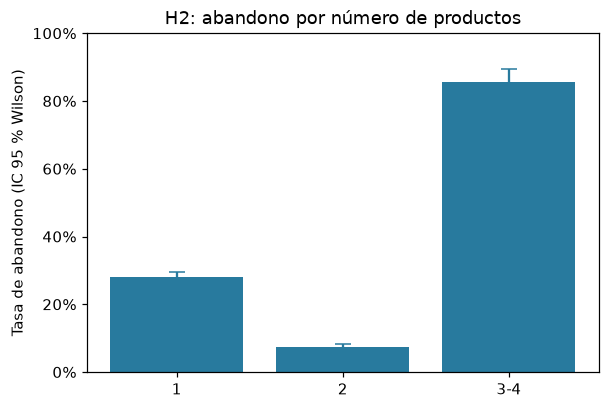
\includegraphics[width=0.82\textwidth]{churn_products.png}
\caption{Relación no monótona con productos, calculada durante la exploración.
Se conserva el grupo pequeño de tres o cuatro productos.}
\end{figure}

\chapter{Pipelines y selección del modelo}
\section{Representaciones y prevención de fuga}
\texttt{FS-RAW} representa las variables candidatas originales; en modelos
lineales las numéricas se escalan. \texttt{FS-EDA} añade el indicador de saldo,
agrupa productos en uno, dos y tres--cuatro mediante one-hot y representa edad
con escalado y término cuadrático. \texttt{FS-TREE} conserva productos y edad
sin esas transformaciones, añade \texttt{has\_balance} y codifica geografía.

Las transformaciones aprendidas se ajustan dentro de un pipeline de
scikit-learn. El componente \texttt{ColumnTransformer} organiza los grupos
de columnas. En cada pliegue se ajustan únicamente con sus filas de entrenamiento.
Los transformadores sin
estado utilizan reglas fijas. \texttt{InputGuard} rechaza columnas reservadas
a auditoría. No se usaron SMOTE, submuestreo ni ponderaciones de clase: la
escala probabilística se conserva antes de calibrar.

\section{Baselines}
En la semana inicial de modelado se compararon tres configuraciones fijas
en cinco pliegues de entrenamiento, sin utilizar validación externa.
\begin{table}[htbp]\centering\small
\caption{Baselines: media y desviación estándar muestral de CV.}
\begin{tabular}{@{}lccc@{}}\toprule
Modelo & AP & ROC-AUC & Brier \\\midrule
Dummy prior & $0{,}204\pm0{,}000$ & $0{,}500\pm0{,}000$ & $0{,}162\pm0{,}000$ \\
LogReg RAW & $0{,}459\pm0{,}029$ & $0{,}755\pm0{,}012$ & $0{,}138\pm0{,}004$ \\
LogReg EDA & $0{,}657\pm0{,}028$ & $0{,}839\pm0{,}021$ & $0{,}111\pm0{,}005$ \\\bottomrule
\end{tabular}
\end{table}
La mejora pareada de AP de EDA frente a RAW fue $0{,}198\pm0{,}019$,
positiva en los cinco pliegues. Es un resumen descriptivo, no una prueba
inferencial entre familias.
\fuente{reports/baselines.md}

\section{Búsqueda y reevaluación}
La FASE A utiliza \texttt{RandomizedSearchCV}, AP, cinco pliegues y semilla 42,
con 20 iteraciones para LogReg y 40 para RF y XGBoost. El máximo de búsqueda
es optimista por selección entre configuraciones. En FASE B, la configuración
ganadora de cada familia se reevalúa con cinco pliegues y dos repeticiones,
semilla 2027 e idénticas particiones entre familias.

\begin{table}[htbp]\centering\small
\caption{Comparación de FASE B, exclusivamente de desarrollo.}\label{tab:faseb}
\begin{tabular}{@{}lccc@{}}\toprule
Familia & AP & ROC-AUC & Brier \\\midrule
LogReg EDA & $0{,}655\pm0{,}027$ & $0{,}839\pm0{,}010$ & $0{,}111\pm0{,}004$ \\
Random Forest & $0{,}686\pm0{,}018$ & $0{,}854\pm0{,}012$ & $0{,}106\pm0{,}003$ \\
XGBoost & $0{,}697\pm0{,}018$ & $0{,}860\pm0{,}010$ & $0{,}106\pm0{,}003$ \\\bottomrule
\end{tabular}
\end{table}

La regla fijada considera cercanos a los candidatos cuya distancia al mejor
promedio sea menor a la desviación estándar del mejor y prioriza LogReg,
después RF y después XGBoost. RF pierde aproximadamente 0,011 de AP frente
a XGBoost, menos que 0,018; se elige RF. Es una heurística de parsimonia,
no una declaración de equivalencia estadística. En validación el candidato
superó a Dummy y a LogReg con AP de 0,696, 0,203 y 0,637, respectivamente.

La configuración final tiene 500 árboles, profundidad máxima 10, mínimo
de cinco observaciones por hoja, \texttt{max\_features="sqrt"}, semilla 42
y \texttt{n\_jobs=-1}.
\fuente{reports/model_selection.md}

\section{Experimentos de variables}
\textbf{E-03:} quitar salario produjo una diferencia pareada de AP de
$+0{,}003\pm0{,}004$. Como supera el límite preregistrado de $-0{,}005$,
se elimina por parsimonia, incluidas sus derivadas.

\textbf{E-02:} quitar productos redujo AP en $0{,}113\pm0{,}021$. Sin quitar
la variable, excluir el pequeño segmento de tres--cuatro productos del cálculo
OOF redujo AP media por repetición de 0,687 a 0,608. El grupo contiene 201 de
los 6\,000 clientes de entrenamiento y es especialmente fácil de separar.
Estas AP agregadas por repetición no se confunden con la media por pliegue
de la tabla~\ref{tab:faseb}. No se promediaron probabilidades entre repeticiones
ni se duplicaron clientes al calcular esas métricas.

\chapter{Calibración y decisión económica}
\section{Probabilidades útiles para decidir}
La AP mide ordenamiento; una campaña basada en valor esperado necesita además
probabilidades interpretables. E-04 genera una predicción OOF para cada fila
de entrenamiento, ajusta calibradores solo con esas predicciones y etiquetas,
y compara en validación la salida original, sigmoide e isotónica.

\begin{table}[htbp]\centering
\caption{Selección de calibración en validación de desarrollo.}
\begin{tabular}{@{}lrrr@{}}\toprule
Variante & Brier & Log loss & AP \\\midrule
Sin calibrar & 0,1026 & 0,3409 & 0,696 \\
Sigmoide & 0,1010 & 0,3361 & 0,696 \\
Isotónica & 0,1013 & 0,3540 & 0,673 \\\bottomrule
\end{tabular}
\end{table}
Se elige sigmoide por menor Brier, con tolerancia de empate de $10^{-4}$.
La implementación usa una regresión logística sin penalización sobre la
probabilidad OOF como única entrada, no sobre etiquetas de validación.
La transformación monótona conserva el orden; la isotónica puede crear empates.
\fuente{reports/decision.md}

\begin{figure}[htbp]\centering
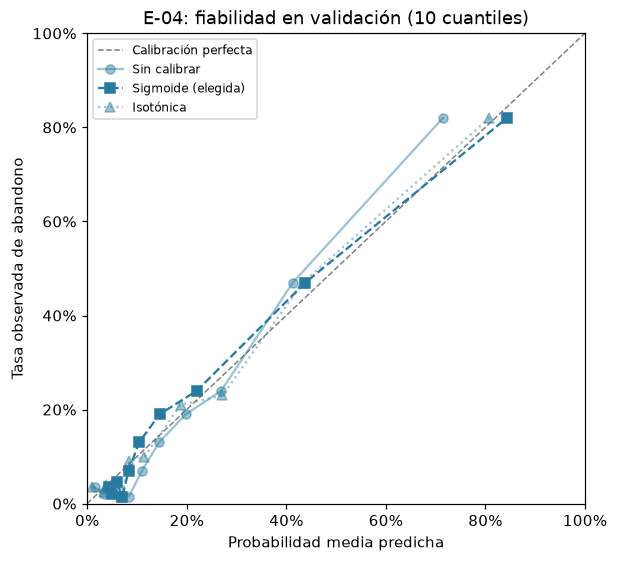
\includegraphics[width=0.85\textwidth]{reliability.png}
\caption{Fiabilidad en validación: diagnóstico de desarrollo de los calibradores.
No es una nueva evaluación en prueba.}
\end{figure}

\section{Derivación del umbral}
Sean $p_i$ la probabilidad calibrada de abandono, $V$ el valor ilustrativo
del cliente, $c$ el coste de contacto y $s$ la eficacia supuesta de retención
en quien iba a abandonar. El valor incremental esperado del contacto es
\begin{equation}
g_i=p_i sV-c.
\end{equation}
La política entregada contacta si el valor es estrictamente positivo:
\begin{equation}\label{eq:umbral}
a_i=\mathbf{1}\{p_i>t^*\},\qquad
t^*=\frac{c}{sV}=\frac{50}{0{,}30\cdot1000}=\frac{1}{6}.
\end{equation}
Con igualdad exacta al umbral no se contacta. El 16,7\,\% mostrado en pantalla
es redondeado; la decisión usa el umbral no redondeado. No se optimizó F1 ni
se buscó un umbral sobre prueba.

\section{Beneficio esperado y evaluación retrospectiva}
Antes de observar etiquetas, la suma de valor esperado de los contactados es
$\sum_i a_i(p_i sV-c)$. Para evaluar una política histórica con etiquetas
$y_i\in\{0,1\}$ se calcula
\begin{equation}\label{eq:beneficio}
B(a)=\sum_i a_i(y_i sV-c).
\end{equation}
Ambas cantidades dependen de los mismos supuestos, pero no son idénticas.
El dashboard de lote muestra valor esperado; los reportes de evaluación
comparan políticas usando etiquetas históricas.

Se supone el mismo valor y eficacia para todos, coste sin efectos secundarios
y beneficio solo si quien iba a abandonar es retenido. No existe evidencia
experimental de $s=0{,}30$. No es posible identificar efecto incremental de
contacto sin datos de tratamiento o un diseño causal apropiado.

\chapter{Evaluación final única}
\section{Protocolo y métricas}
El 7 de octubre de 2026 se evaluó una sola vez el artefacto congelado sobre
2\,000 clientes de prueba, con 407 abandonos. Se fijaron antes variables,
pipeline, hiperparámetros, calibrador, supuestos y umbral. La corrida MLflow
registra \texttt{stage=final} y \texttt{final=true}. La existencia del reporte
y la metadata completada bloquean una repetición mediante la CLI normal.

La precisión promedio se calcula como $\mathrm{AP}=\sum_k(R_k-R_{k-1})P_k$;
no es la integración trapezoidal de la curva precisión--sensibilidad. Brier
es el promedio $(p_i-y_i)^2$ y log loss penaliza probabilidades incorrectas
con alta confianza. ROC-AUC resume ordenamiento global sin fijar umbral.

\begin{table}[htbp]\centering
\caption{Resultados finales del reporte congelado.}\label{tab:final}
\begin{tabular}{@{}lr@{}}\toprule
Métrica & Valor \\\midrule
AP & 0,704671 \\
ROC-AUC & 0,861620 \\
Brier & 0,101683 \\
Log loss & 0,337974 \\
Probabilidad media & 20,5006\,\% \\
Abandono observado & 20,35\,\% \\
Precisión en $t^*$ & 49,0536\,\% \\
Sensibilidad en $t^*$ & 76,4128\,\% \\
F1 en $t^*$ & 0,597502 \\\bottomrule
\end{tabular}
\end{table}
La cercanía entre probabilidad media y prevalencia es un diagnóstico global,
no una garantía de calibración en cada segmento. El hecho de que AP de prueba
sea próxima a AP de validación no prueba ausencia de sobreajuste; es compatible
con una generalización similar en esta partición.

\section{Políticas y matriz de confusión}
\begin{table}[htbp]\centering\small
\caption{Comparación retrospectiva bajo los supuestos fijados, en EUR.}
\begin{tabular}{@{}lrrr@{}}\toprule
Política & Contactados & Abandonos captados & Beneficio \\\midrule
Nadie & 0 & 0 & 0 \\
Todos & 2\,000 & 407 & 22\,100 \\
Aleatoria 20\,\% & 400 & 81,4 & 4\,420 \\
Modelo & 634 & 311 & 61\,600 \\
Oráculo & 407 & 407 & 101\,750 \\\bottomrule
\end{tabular}
\end{table}
La fila aleatoria es un valor esperado, por eso puede contener un número
fraccionario de abandonos captados; no es una campaña simulada concreta.
El oráculo conoce las etiquetas y es una cota ideal bajo los supuestos, no
una política desplegable. El modelo mejora en 39\,500 EUR a la mejor referencia
sin modelo y alcanza el 60,54\,\% de esa cota.

La matriz en el umbral económico tiene VN=1\,270, FP=323, FN=96 y VP=311.
Como control aritmético, $311\cdot300-634\cdot50=61\,600$. Las 634 decisiones
positivas corresponden a $311+323$, coherentes con la tabla. Esta lectura del
reporte existente no implica otra ejecución sobre los datos de prueba.
\fuente{reports/final_test.json}

\chapter{Explicabilidad, errores y equidad}
\section{Alcance de SHAP}
SHAP explica la probabilidad \emph{sin calibrar} del Random Forest base.
La auditoría comprobó aditividad con error máximo de $9{,}3\times10^{-15}$.
La API devuelve tres contribuciones locales con signo; el dashboard las
expresa en puntos porcentuales sin calibrar. No suman necesariamente a la
probabilidad calibrada que se muestra al usuario y no son causas.

Edad, productos, actividad y la categoría Alemania dominan la importancia
global. Por su señal compartida se reportan también grupos de saldo y
geografía; repartir contribuciones entre variables correlacionadas no establece
una explicación causal independiente para cada una.
\begin{figure}[htbp]\centering
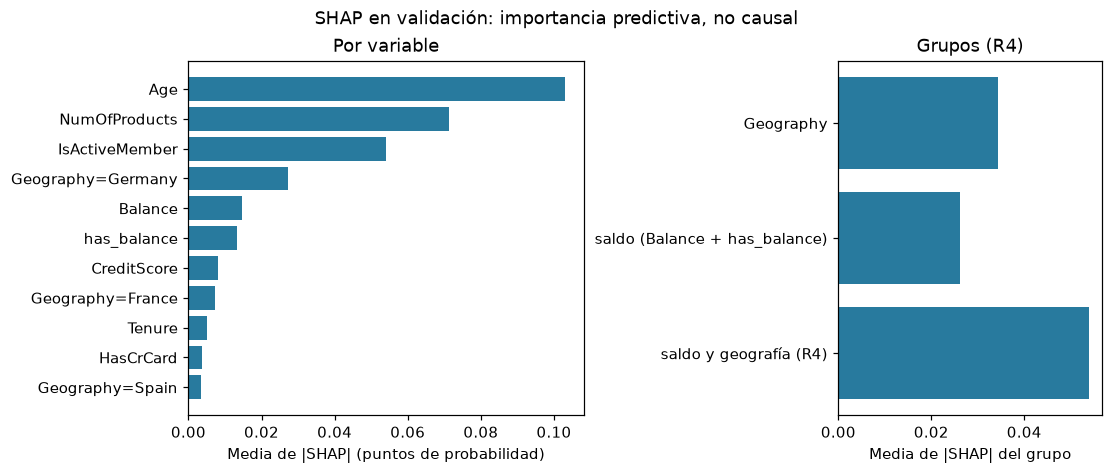
\includegraphics[width=0.85\textwidth]{shap_importance.png}
\caption{Importancia SHAP global de la auditoría en validación.}
\end{figure}

\section{Errores y segmentos}
En validación los falsos negativos tienen menor edad media y mayor proporción
de actividad que los verdaderos positivos. El grupo de 18--29 años dejó sin
contactar al 65,4\,\% de sus 26 abandonos. Una banda de $\pm0{,}05$ alrededor
de $t^*$ contiene 319 clientes; cambios de supuestos podrían alterar decisiones
en esa zona. Son diagnósticos de desarrollo: no se ajustó la política a partir
de esos casos ni se transfirieron esas cifras a prueba.

\section{E-01: auditoría por género}
\texttt{Gender} se conserva exclusivamente para análisis de segmentos. La
auditoría de validación contiene 889 mujeres y 1\,111 hombres. La condición
de alerta preregistrada exige un IC de diferencia que excluya cero y una
magnitud absoluta de al menos cinco puntos porcentuales.
\begin{table}[htbp]\centering\small
\caption{E-01 en validación: porcentajes e IC de diferencia en pp.}
\begin{tabular}{@{}lrrrl@{}}\toprule
Métrica & Mujeres & Hombres & IC de F--M & Alerta \\\midrule
Contacto & 31,2 & 31,0 & [$-3{,}9$;4,4] & No \\
Sensibilidad & 77,5 & 74,7 & [$-5{,}7$;10,9] & No \\
Precisión & 59,6 & 42,2 & [10,3;25,2] & Sí \\
Brecha de calibración & $-1{,}8$ & 1,9 & [$-6{,}7$;$-0{,}9$] & No \\\bottomrule
\end{tabular}
\end{table}
La diferencia de precisión es aproximadamente 17,4 pp y coincide con tasas
base distintas, 24,0\,\% y 17,5\,\%. La diferencia de calibración tiene IC sin
cero, pero su magnitud puntual no supera el umbral práctico de alerta. Que
contacto y sensibilidad no disparen alerta no demuestra igualdad ni elimina
riesgos de discriminación. Excluir género no garantiza equidad. No se entrenó
una variante con género ni se aplicó mitigación en esta entrega.
\fuente{reports/audit.md}

\chapter{Monitoreo simulado}
\section{Diseño de escenarios}
La referencia es entrenamiento y la población actual se construye con
validación, usando semilla 2028. Se evalúan S0, control sin cambio; S1,
envejecimiento; S2, doble proporción alemana; S3, 70\,\% de inactivos; y S4,
35\,\% de abandono mediante remuestreo por etiqueta. No se utiliza prueba.

Para proporciones de intervalos de referencia $r_b$ y actuales $q_b$, PSI
resume el desplazamiento como $\sum_b(q_b-r_b)\log(q_b/r_b)$, con el tratamiento
de bins y proporciones pequeñas fijado en la implementación. Es una medida
descriptiva dependiente de la discretización, no un p-valor. Se considera estable
por debajo de 0,10, moderado hasta 0,25 y alarma estrictamente por encima de
0,25. KS y chi-cuadrado con Holm son apoyo estadístico.

La degradación se define antes de simular: brecha entre probabilidad media y
abandono observado fuera de $\pm3$ pp, o Brier mayor que 1,15 veces S0. Brier
depende de la composición de clientes; un aumento no identifica por sí solo
un deterioro condicional del modelo.

\begin{table}[htbp]\centering\small
\caption{Síntesis de escenarios: señales y degradación.}
\begin{tabular}{@{}lrrrrl@{}}\toprule
Escenario & PSI desplazado & Contacto (\%) & Brecha (pp) & Brier & Degrada \\\midrule
S0 & --- & 31,1 & +0,3 & 0,1010 & No \\
S1 & Edad: 0,327 & 42,2 & +1,4 & 0,1100 & No \\
S2 & Geografía: 0,275 & 38,2 & $-0{,}7$ & 0,1191 & Sí \\
S3 & Actividad: 0,196 & 34,9 & $-0{,}1$ & 0,1030 & No \\
S4 & Máximo entradas: 0,023 & 38,6 & $-9{,}6$ & 0,1418 & Sí \\\bottomrule
\end{tabular}
\end{table}

\section{Expectativas y aprendizaje}
E1 se cumplió: S0 no presenta alarma ni degradación. E2 no se cumplió:
S1 y S2 sí disparan alarma en la variable desplazada, pero S3 permanece en
PSI 0,196. Se conserva el umbral original, sin retocarlo para lograr éxito.
E3 se cumplió: S4 no dispara alarma de entradas, pero descalibra en $-9{,}6$
pp. E4 se cumplió: la tasa de contacto se separa más de dos pp del control
en los cuatro escenarios alterados.

La conclusión operativa es que vigilar entradas no sustituye el seguimiento
de resultados con etiquetas. Las tasas de contacto pueden ser una señal
temprana, pero no bastan para establecer calibración. Son simulaciones sobre
validación ya utilizada; no constituyen monitoreo de clientes reales.
\fuente{reports/monitoring.md}
\begin{figure}[htbp]\centering
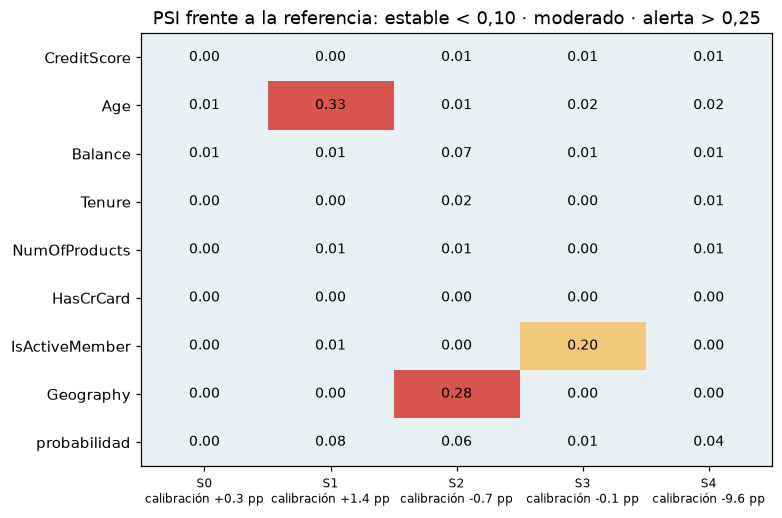
\includegraphics[width=0.95\textwidth]{monitoring_psi.png}
\caption{PSI por variable y escenario en la simulación preregistrada.}
\end{figure}

\chapter{Arquitectura y contratos de aplicación}
\section{Separación de responsabilidades}
El dashboard presenta resultados, pero no carga el artefacto ni ejecuta
predicciones propias. FastAPI concentra validación, inferencia, razones y
regla económica. El modelo, metadata y explicador se cargan al arrancar,
una vez por proceso. Los reportes finales y de monitoreo son agregados ya
generados; consultarlos no repite sus experimentos.

\begin{figure}[htbp]\centering
\begin{tikzpicture}[node distance=0.7cm and 0.8cm,
 box/.style={draw=azul,rounded corners,align=center,minimum height=1.1cm,
 text width=3.3cm,fill=fondo,font=\small},arr/.style={-{Latex},thick}]
\node[box] (u) {Usuario\\navegador HTTPS};
\node[box,right=of u] (st) {Streamlit\\interfaz y sesión};
\node[box,right=of st] (api) {FastAPI interna\\contrato e inferencia};
\node[box,below=of api] (model) {RF + sigmoide\\política $p>1/6$ y SHAP};
\node[box,below=of st] (release) {Release del modelo\\descarga y SHA-256};
\draw[arr] (u)--(st); \draw[arr] (st)--node[above,font=\scriptsize]{HTTP} (api);
\draw[arr] (api)--(model); \draw[arr] (release)--(model);
\end{tikzpicture}
\caption{Flujo de la instancia Render: únicamente Streamlit es público.}
\end{figure}

\section{API}
El contrato Pydantic prohíbe extras y números no finitos. La tabla
\ref{tab:contrato} resume sus ocho entradas predictivas.
\begin{longtable}{@{}L{0.32\textwidth}L{0.58\textwidth}@{}}
\caption{Endpoints del servicio FastAPI.}\\
\toprule Ruta & Comportamiento \\\midrule\endfirsthead
\toprule Ruta & Comportamiento \\\midrule\endhead
\texttt{GET /health} & Estado, SHA-256 del artefacto y commit del modelo. \\
\texttt{GET /model} & Variables, umbral, supuestos y agregados históricos de prueba. \\
\texttt{POST /predict} & Probabilidad, decisión, valor esperado, umbral y tres razones. \\
\texttt{POST /predict/batch} & Hasta 1\,000 clientes; predicciones y resumen de contactos. \\
\texttt{POST /explain} & Predicción y explicación textual con origen de la explicación. \\
\texttt{GET /monitoring} & Reporte existente; 404 si no está disponible. \\
\bottomrule
\end{longtable}
En Render estos endpoints están en loopback, no expuestos como API pública.
La documentación interactiva se consulta en el servicio local, en
\url{http://localhost:8000/docs}. El resumen de lote suma valor esperado solo
de quienes se recomienda contactar; el valor individual puede ser negativo.

\section{Dashboard y estado}
Las vistas laterales son Cliente, Lote, Modelo y Monitoreo. Cliente requiere
una acción explícita; permite cargar el perfil sintético de referencia y
muestra probabilidad, umbral, decisión y factores. Lote valida el CSV antes
de procesar y presenta distribución de riesgo, contactos y exportación.
Modelo muestra los agregados congelados y Monitoreo las simulaciones.

Los perfiles y resultados viven en \texttt{st.session\_state}, no en una
caché global compartida. Cada resultado individual conserva el perfil que
se evaluó; editar un formulario no convierte el resultado anterior en una
inferencia nueva. Cambiar el contenido normalizado del lote invalida su
resultado, mientras navegar, filtrar o descargar no reenvía predicciones.
El único recurso global compartido es el transporte HTTP de la API.

\chapter{Seguridad y despliegue}
\section{Controles de consumo y datos}
La instancia usa un único worker de API. Los límites globales aprobados son
60 intentos de inferencia por minuto, dos simultáneos y cuerpo JSON de hasta
512 KiB. La interfaz limita CSV a 1 MiB y 1\,000 filas. Frecuencia y concurrencia
devuelven HTTP 429 con \texttt{Retry-After}; tamaño excesivo devuelve 413.

La exportación conserva únicamente las entradas normalizadas y las salidas.
Descarta género, identificadores, apellidos, salario y columnas extra; protege
además texto con prefijos de fórmula. El texto explicativo se representa
literalmente. Los errores de validación no devuelven valores rechazados.
Los datos reales y las credenciales no entran en Git, la imagen ni el contexto HF.

\section{Cabeceras y transporte}
El launcher \path{dashboard/serve.py} utiliza la API pública
\texttt{st.App} de Streamlit y middleware ASGI sin buffer. Añade las cabeceras
del cuadro siguiente sin consumir cuerpos ni modificar WebSocket o lifespan.
\begin{table}[htbp]\centering\small
\caption{Cabeceras del dashboard público.}
\begin{tabularx}{\textwidth}{@{}lX@{}}\toprule
Cabecera & Valor \\\midrule
\texttt{X-Content-Type-Options} & \texttt{nosniff} \\
\texttt{Referrer-Policy} & \texttt{no-referrer} \\
\texttt{Strict-Transport-Security} & \texttt{max-age=31536000} \\
\texttt{X-Frame-Options} & \texttt{SAMEORIGIN} \\
\texttt{Content-Security-Policy} & \texttt{frame-ancestors 'self'} \\\bottomrule
\end{tabularx}
\end{table}
HSTS no incluye subdominios ni preload. La CSP descrita cubre framing, no
una política exhaustiva de contenido. CORS y XSRF permanecen activos. La
cookie XSRF se observa también en el endpoint de salud, sin registrar su valor.
En la prueba pública se observó SameSite Lax; la política comprobada exige
Secure si se configura SameSite None, no HttpOnly al token leído por el cliente.

\section{LLM opcional}
La explicación generativa necesita un proveedor compatible con OpenAI. Solo
recibe hechos de las variables permitidas y razones; no identificadores ni
género. Un error, timeout o agotamiento de presupuesto produce una plantilla
determinista. El presupuesto por defecto es 30 intentos por hora e incluye
fallidos; SQLite permite compartirlo entre procesos de la misma instancia.
No es un limitador distribuido entre hosts.

En Render Free el LLM está desactivado mediante
\texttt{LLM\_MAX\_CALLS\_PER\_HOUR=0}; el disco es efímero y no se presenta
esa cuota como persistencia entre reemplazos de instancia. La demo final
respondió con plantilla, comprobada en navegador real.

\section{Docker, artefacto y Render}
El build descarga \texttt{model.joblib} de \texttt{model-v1.0}; el SHA-256
se comprueba antes de deserializar y un desacuerdo detiene la carga. El
Dockerfile fija las imágenes base por digest y usa usuario sin privilegios.
Solo el estado de ejecución es escribible por el usuario del servicio.

Render ejecuta una imagen con \texttt{ROLE=all}, API interna en
\url{http://127.0.0.1:8000} y dashboard en el puerto 10\,000. El servicio
Free se limita a 512 MiB y 0,1 CPU; Auto-Deploy está desactivado y se despliega
manualmente después de CI verde. El health público es
\texttt{/\_stcore/health}, diferente de \texttt{/health} de la API.
Hugging Face se conserva como alternativa manual, no como requisito de entrega.

El mensaje de consola que anuncia una URL no demuestra que el navegador ya
pueda abrirla. Tras inactividad Render Free puede mostrar
\textit{Application loading} mientras despierta. La verificación funcional
se ejecuta después de obtener health correcto, no contra esa pantalla transitoria.

\chapter{Reproducibilidad, pruebas y operación}
\section{Trazabilidad de artefactos}
El modelo es un pipeline más calibrador y metadata. Su identidad no depende
del nombre local del archivo sino del hash esperado:
\begin{lstlisting}
579b7fe349dc035c3171582cbfba1bfaed4599a795da4b149d7664ed21dc095a
\end{lstlisting}
\texttt{model-v1.0} identifica el artefacto; \texttt{v1.0.1} la entrega de
código. El commit de entrenamiento es distinto al commit de serving; no se
actualiza la procedencia histórica para hacerla coincidir artificialmente.
La metadata conserva versiones, variables, hiperparámetros y hashes.

MLflow registra parámetros, métricas, semilla, particiones, commit y hashes.
La base local no se versiona. El manifiesto de las fases iniciales conservó
hashes de bytes sensibles al fin de línea; desde calibración se registra
hash canónico del JSON. Diferencias históricas CRLF/LF no implican por sí
solas una división diferente.

\section{Pruebas y CI}
Los tests utilizan datos sintéticos y tracking temporal. Cubren contratos,
transformaciones, selección, decisiones, guardas de prueba única, API,
cuota, límites, empaquetado, interfaz y transporte de cabeceras. La última
suite local de la entrega aprobó 322 tests con cobertura 98,19\,\%. En clon
sin datos ni artefacto locales fueron 319 aprobados y tres omitidos esperados,
con 98,11\,\%. Son ejecuciones distintas y no se suman entre sí.

CI ejecuta sincronización bloqueada, Ruff y pytest con cobertura mínima del
85\,\%. Un workflow separado audita dependencias y secretos; falla si detecta
hallazgos o no puede completar el análisis. Se fijan Actions por SHA y se
minimizan los informes de secretos. Los resultados de una plataforma no
certifican todas las combinaciones posibles de Python y sistema operativo.

\section{Verificación de la entrega}
La Release documenta un único commit nuevo de cierre, \texttt{\versioncodigo},
integrado por avances rápidos de los PR 2 y 1. CI y Security scans de
\texttt{main} fueron satisfactorios. El responsable aportó captura del deploy
Live del mismo commit y duración de 2 min 14 s; las pruebas HTTPS y de
navegador se realizaron independientemente sobre la URL real.

La auditoría HTTP devolvió código cero: TLS, redirección, cabeceras, health,
cookie y WebSocket propio 101/ajeno 403. Edge aprobó doce controles funcionales,
sin errores de consola, con lote de 20 perfiles sintéticos y descarga de 20
filas/11 columnas. Una prueba adicional confirmó subida válida 204 y sin
token XSRF 403. La revisión de escritorio/móvil/reflow no certifica WCAG
completa ni capacidad bajo carga productiva.

La imagen de referencia también se comprobó localmente con 512 MiB, sin
swap adicional y 0,1 CPU, sin OOM. El build y Compose desde un clon limpio
descargaron el modelo y terminaron satisfactoriamente. Esto no transforma
una medición local en garantía de rendimiento de toda carga pública.

\section{Manual de operación y recuperación}
\begin{enumerate}
\item Para abrir la demo, utilizar la URL de Render y esperar el arranque en frío.
\item Ante una interfaz anterior, comprobar el commit Live y la rama del servicio;
  un push no despliega si Auto-Deploy está Off.
\item Ante fallo de salud, revisar logs de build/arranque y puerto público.
  FastAPI debe seguir en loopback; no sustituir el health de Streamlit por el suyo.
\item Ante hash incorrecto, conservar el rechazo y revisar el asset de la Release.
  No relajar la verificación para forzar el arranque.
\item Ante CSV inválido, corregir columnas/rangos/UTF-8 o partir el lote; no elevar
  límites automáticamente para salvar una carga.
\item Para actualizar código, comprobar CI, desplegar manualmente y repetir
  auditoría y recorrido. Conservar la identidad del modelo si no se autoriza otro.
\end{enumerate}

\chapter{Estado de Git, conclusiones y evolución}
\section{Higiene del repositorio}
La auditoría documental del 15 de octubre confirmó una única rama local y
remota, \texttt{main}, en \texttt{\versioncodigo}, sin cambios pendientes antes
de añadir esta memoria. Los dos PR están fusionados. Se preservan las etiquetas
\texttt{model-v1.0}, \texttt{v1.0.0} y \texttt{v1.0.1}; la segunda es anterior
al cierre público y no se mueve para ocultar esa secuencia.

No se versionan CSV reales, modelo, MLflow, entorno, cachés ni salidas de
compilación. El CSV de ejemplo es sintético y sí es un artefacto intencional.
El stash \texttt{render-prep} se conserva como propuesta histórica apartada;
no forma parte de la entrega aceptada ni del working tree. Los planes y
reportes se conservan por trazabilidad, no se clasifican como basura por edad.

\section{Conclusiones}
\begin{enumerate}
\item La calidad del ranking y la calibración cumplen funciones distintas.
  Un umbral económico necesita probabilidades y supuestos interpretables.
\item La selección y las expectativas preregistradas permiten informar
  resultados desfavorables, como E2, sin reinterpretar criterios después.
\item La ausencia de género en las entradas no elimina diferencias de resultados;
  la auditoría identifica una brecha de precisión que debe permanecer visible.
\item El monitoreo de entradas no detecta necesariamente degradación por cambio
  de prevalencia. Una operación real necesita etiquetas y evaluación continua.
\item La entrega técnica requiere evidencia de código, CI, artefacto y servicio
  público. Un estado Live o una URL en consola no sustituyen esa comprobación.
\end{enumerate}

\section{Trabajo futuro}
Las extensiones requieren otro diseño: presupuesto por deciles, sensibilidad
de $V,c,s$, valor heterogéneo por cliente, tratamiento causal, mitigación de
E-01 y monitoreo con etiquetas reales. Una adaptación institucional exige
revalidar contrato, procedencia, horizonte temporal y población, además de
autenticación, protección de datos y objetivos operativos propios. No se
promete trasladar las métricas actuales sin esa validación.

\appendix
\chapter{Uso local y ejemplos}
\section{Instalación y demo}
Los comandos siguientes son instrucciones, no ejecuciones realizadas al
redactar la memoria. Desde la raíz del repositorio, con Git y uv instalados:
\begin{lstlisting}
uv sync --locked
uv run python -m churn.artifact
# Terminal 1
uv run uvicorn churn.api:app --host 127.0.0.1 --port 8000
# Terminal 2
uv run streamlit run dashboard/serve.py
\end{lstlisting}
En PowerShell se desactiva el proveedor antes de arrancar la API:
\begin{lstlisting}
$env:LLM_MAX_CALLS_PER_HOUR = "0"
\end{lstlisting}
La alternativa Docker se inicia con el siguiente comando. Sus puertos locales
son 8000 para API y 8501 para dashboard, publicados en loopback.
\begin{lstlisting}
docker compose up --build
\end{lstlisting}

\section{Cliente ilustrativo de referencia}
\begin{lstlisting}
{
  "CreditScore": 600,
  "Age": 52,
  "Tenure": 3,
  "Balance": 120000,
  "NumOfProducts": 1,
  "HasCrCard": 1,
  "IsActiveMember": 0,
  "Geography": "Germany"
}
\end{lstlisting}
Su probabilidad de referencia es aproximadamente 0,9470014742 y se recomienda
contactar. El valor esperado individual bajo los supuestos es aproximadamente
234,10 EUR; la interfaz lo redondea. Para lotes, el cuerpo es un objeto con
clave \texttt{customers} y una lista de objetos del mismo contrato.

\section{Comprobaciones de desarrollo}
\begin{lstlisting}
uv sync --locked
uv run ruff check .
uv run ruff format --check .
uv run pre-commit run --all-files
uv run pytest --cov=churn --cov-report=term-missing --cov-fail-under=85
python scripts/verify_public_security.py --url https://bank-churn-ml-ufa7.onrender.com/
\end{lstlisting}
La auditoría devuelve 0 si pasa, 1 ante fallo comprobado y 2 si la evidencia
no pudo verificarse. Un timeout de arranque no se convierte en un aprobado.
Los comandos de entrenamiento y \texttt{churn-final} no forman parte de esta
comprobación de entrega; no deben ejecutarse para regenerar la documentación.

\chapter{Mapa de fuentes y entrega}
\begin{longtable}{@{}L{0.42\textwidth}L{0.48\textwidth}@{}}
\caption{Fuentes primarias utilizadas por esta memoria.}\\
\toprule Fuente & Contenido \\\midrule\endfirsthead
\toprule Fuente & Contenido \\\midrule\endhead
\path{specs/001-007} & Diseño y enmiendas; consultar los nombres completos del directorio. \\
\path{reports/data_quality.json} & Calidad global inicial. \\
\path{reports/eda_hypotheses.md} & Hipótesis y exploración de entrenamiento/validación. \\
\path{reports/baselines.md} & Baselines de cinco pliegues. \\
\path{reports/model_selection.md} & FASE A/B y E-02/E-03. \\
\path{reports/decision.md} & E-04 y política económica de desarrollo. \\
\path{reports/final_test.json} & Evaluación final única y políticas retrospectivas. \\
\path{reports/audit.md} & SHAP, errores, segmentos y E-01. \\
\path{reports/monitoring.md} & Simulaciones S0--S4 y expectativas E1--E4. \\
\path{reports/model_metadata.json} & Configuración y procedencia del artefacto. \\
\path{src/churn/api.py} & Contratos y respuestas HTTP implementados. \\
\path{docs/registro-avance.md} & Evidencia cronológica y limitaciones de comprobación. \\
Release \texttt{v1.0.1} & Cierre público posterior al snapshot S24 e informe JSON de verificación. \\
\bottomrule
\end{longtable}

Código documentado completo:
\begin{lstlisting}
9384e51e22b069d0bab4ae58b6be9920d97d68f0
\end{lstlisting}
La memoria es una ampliación documental posterior. No atribuye su propia
fuente LaTeX a un commit histórico que todavía no la contenía. El PDF se
compila a \path{docs/latex/build/}; su fuente e instrucciones están separadas
de los auxiliares regenerables para mantener limpio Git.

\begin{thebibliography}{10}
\addcontentsline{toc}{chapter}{Bibliografía y referencias de consulta}
\bibitem{repo} Jacome Cuenca, D. \textit{bank-churn-ml, entrega v1.0.1}.
Código, reportes y evidencia: \url{https://github.com/darwinjaco/bank-churn-ml/releases/tag/v1.0.1}.
\bibitem{kaggle} Kaggle. \textit{Churn Modelling}, fuente declarada del dataset.
\url{https://www.kaggle.com/datasets/shrutimechlearn/churn-modelling}.
\bibitem{sklearn} scikit-learn. Documentación de pipelines, validación cruzada,
calibración y métricas. \url{https://scikit-learn.org/stable/}.
\bibitem{shap} SHAP. Documentación de explicaciones de modelos.
\url{https://shap.readthedocs.io/}.
\bibitem{mlflow} MLflow. Documentación de seguimiento de experimentos.
\url{https://mlflow.org/docs/latest/}.
\bibitem{fastapi} FastAPI. Documentación del framework.
\url{https://fastapi.tiangolo.com/}.
\bibitem{streamlit} Streamlit. Documentación de aplicaciones y configuración.
\url{https://docs.streamlit.io/}.
\bibitem{render} Render. Características y límites de servicios gratuitos.
\url{https://render.com/docs/free}.
\bibitem{tectonic} Tectonic. Compilador utilizado para validar la memoria.
\url{https://tectonic-typesetting.github.io/}.
\end{thebibliography}
\end{document}
